\documentclass[aspectratio=169]{beamer}
\usetheme{Madrid}
\usecolortheme{default}
\usepackage[utf8]{inputenc}
\usepackage[T5]{fontenc}
\usepackage{graphicx}
\usepackage{hyperref}
\usepackage{booktabs}
\usepackage{amsmath}
\usepackage{listings}
\usepackage{xcolor}

\setbeamertemplate{caption}[numbered]
\renewcommand{\figurename}{Hình}
\renewcommand{\thefigure}{9.\arabic{figure}}

% Cấu hình listings cho Python
\definecolor{codegreen}{rgb}{0,0.6,0}
\definecolor{codegray}{rgb}{0.5,0.5,0.5}
\definecolor{codepurple}{rgb}{0.58,0,0.82}
\definecolor{backcolour}{rgb}{0.95,0.95,0.92}

\lstdefinestyle{mystyle}{
    backgroundcolor=\color{backcolour},   
    commentstyle=\color{codegreen},
    keywordstyle=\color{magenta},
    numberstyle=\tiny\color{codegray},
    stringstyle=\color{codepurple},
    basicstyle=\ttfamily\scriptsize,
    breakatwhitespace=false,         
    breaklines=true,                 
    captionpos=b,                    
    keepspaces=true,                 
    numbers=left,                    
    numbersep=5pt,                  
    showspaces=false,                
    showstringspaces=false,
    showtabs=false,                  
    tabsize=2
}
\lstset{style=mystyle}

\title[Chương 9: Kiến trúc ConvNet]{Học Sâu (Deep Learning) \\ \vspace{0.5cm} \Large Chương 9: Các Mẫu Kiến trúc Mạng Tích chập \\ (ConvNet Architecture Patterns)}
\author{Đại học Đông Á}
\date{\today}

\begin{document}

\begin{frame}
    \titlepage
\end{frame}

\begin{frame}{Nội dung chương}
    \tableofcontents
\end{frame}

\section{1. Nguyên lý Thiết kế Kiến trúc}

\begin{frame}{Không gian Giả thuyết (Hypothesis Space)}
    \begin{itemize}
        \item \textbf{Kiến trúc Mô hình (Model Architecture)} là nghệ thuật lắp ráp các tầng mạng (Layers).
        \item Cấu trúc này định nghĩa \textbf{Không gian Giả thuyết} (Hypothesis Space). Thuật toán Gradient Descent sẽ tìm kiếm bộ tham số (Weights) tối ưu bên trong không gian này.
        \item Một kiến trúc tốt giống như một bản thiết kế thông minh, giúp đóng gói \textbf{Tri thức tiên nghiệm (Prior Knowledge)} của kỹ sư vào mô hình.
        \item Ví dụ: Việc sử dụng Tích chập (Convolution) thay cho mạng Dense hàm chứa tri thức tiên nghiệm rằng: \textit{"Các mẫu cục bộ trong hình ảnh là bất biến với sự dịch chuyển"}.
    \end{itemize}
\end{frame}

\begin{frame}{Tầm quan trọng của Thiết kế Kiến trúc}
    \begin{itemize}
        \item Thiết kế khéo léo sẽ làm \textbf{thu hẹp không gian tìm kiếm}, giúp Gradient Descent hội tụ nhanh hơn về điểm tối ưu.
        \item Nó cũng giúp mô hình sử dụng dữ liệu hiệu quả hơn, chống lại hiện tượng Overfitting ngay cả khi tập dữ liệu huấn luyện khá nhỏ.
        \item Ngược lại, nếu chọn một kiến trúc sai lầm (ví dụ: dùng mạng Dense để nhận diện ảnh 4K), mô hình sẽ mãi mắc kẹt ở hiệu suất thấp, và không có một lượng dữ liệu lớn nào có thể cứu vãn được.
    \end{itemize}
\end{frame}

\begin{frame}{Nghệ thuật Thiết kế vs. Bằng chứng Khoa học}
    \begin{itemize}
        \item Thiết kế kiến trúc thường nghiêng về \textbf{Nghệ thuật (Art)} hơn là Khoa học chính xác (Science).
        \item Các kỹ sư máy học xuất chúng thường sử dụng \textbf{Trực giác (Intuition)} và kinh nghiệm nhận dạng mẫu (Pattern Matching) để ghép nối mô hình, thay vì dựa vào các chứng minh toán học khắt khe.
        \item Sự thật: Không ai có thể giải thích bằng toán học một cách hoàn hảo \textit{tại sao} một kiến trúc lại hoạt động tốt hơn kiến trúc khác. Ta chỉ biết nó hiệu quả thông qua thực nghiệm.
    \end{itemize}
\end{frame}

\begin{frame}{Ablation Studies (Nghiên cứu Cắt bỏ)}
    \begin{itemize}
        \item Trong bối cảnh ngành Deep Learning có nhiều cấu trúc phức tạp được công bố chỉ để làm bài báo trông "nguy hiểm" hơn (Tối ưu hóa cho Peer Review).
        \item Mục tiêu thực sự của kỹ sư là \textbf{Tìm hiểu quan hệ Nhân quả}.
        \item \textbf{Ablation Studies:} Kỹ thuật gỡ bỏ từng thành phần của mô hình để kiểm chứng xem sự phức tạp được thêm vào có thực sự mang lại hiệu quả không.
        \item \textit{Ví dụ:} Nếu mô hình X + Y + Z hoạt động tốt, hãy thử chạy lại với chỉ X, Y, Z, X+Y... để biết chính xác sức mạnh đến từ đâu.
    \end{itemize}
\end{frame}

\begin{frame}{Công thức MHR: Modularity, Hierarchy, Reuse}
    \begin{columns}
        \column{0.5\textwidth}
        Để quản lý một hệ thống phức tạp, ta dùng nguyên lý \textbf{MHR}:
        \begin{itemize}
            \item \textbf{Modularity (Mô-đun hóa):} Đóng gói các lớp tính toán cơ bản thành các Khối (Blocks) độc lập.
            \item \textbf{Hierarchy (Phân cấp):} Xếp chồng các khối thành hệ thống hình Tháp (Pyramid).
            \item \textbf{Reuse (Tái sử dụng):} Tái sử dụng cùng một cấu trúc khối lặp đi lặp lại.
        \end{itemize}
        
        \column{0.5\textwidth}
        \begin{figure}
            \centering
            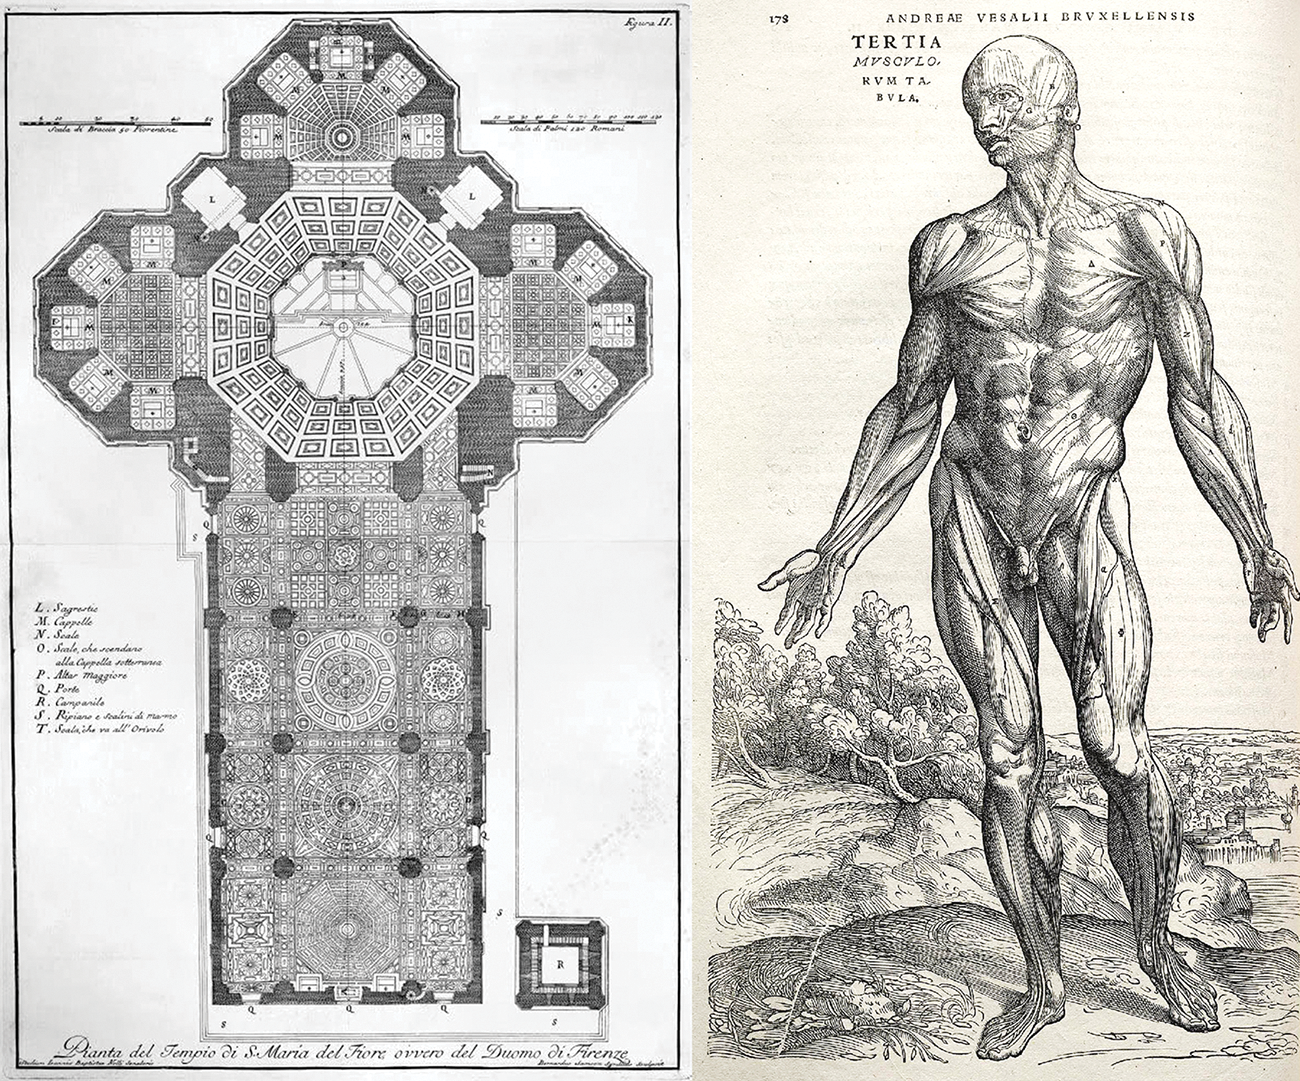
\includegraphics[width=\textwidth,height=0.6\textheight,keepaspectratio]{../../images/ch09/complex_systems.e89aaf78.png}
            \caption{Hệ thống phức tạp sinh học tuân theo nguyên lý MHR}
        \end{figure}
    \end{columns}
\end{frame}

\begin{frame}{Tháp Đặc trưng trong Mô hình Xception}
    \begin{columns}
        \column{0.5\textwidth}
        \begin{itemize}
            \item Các mạng CNN hiện đại (như Xception, ResNet) tuân thủ chặt chẽ nguyên lý MHR.
            \item Cấu trúc Lặp lại (Reuse): Khối \texttt{SeparableConv} $\rightarrow$ \texttt{SeparableConv} $\rightarrow$ \texttt{MaxPooling}.
            \item \textbf{Tháp không gian:} Kích thước bản đồ giảm dần (Shrinking: $299 \times 299 \rightarrow 19 \times 19$).
            \item \textbf{Tháp chiều sâu:} Số lượng bộ lọc (Filters) tăng dần (Deepening: $32 \rightarrow 728$).
        \end{itemize}
        
        \column{0.5\textwidth}
        \begin{figure}
            \centering
            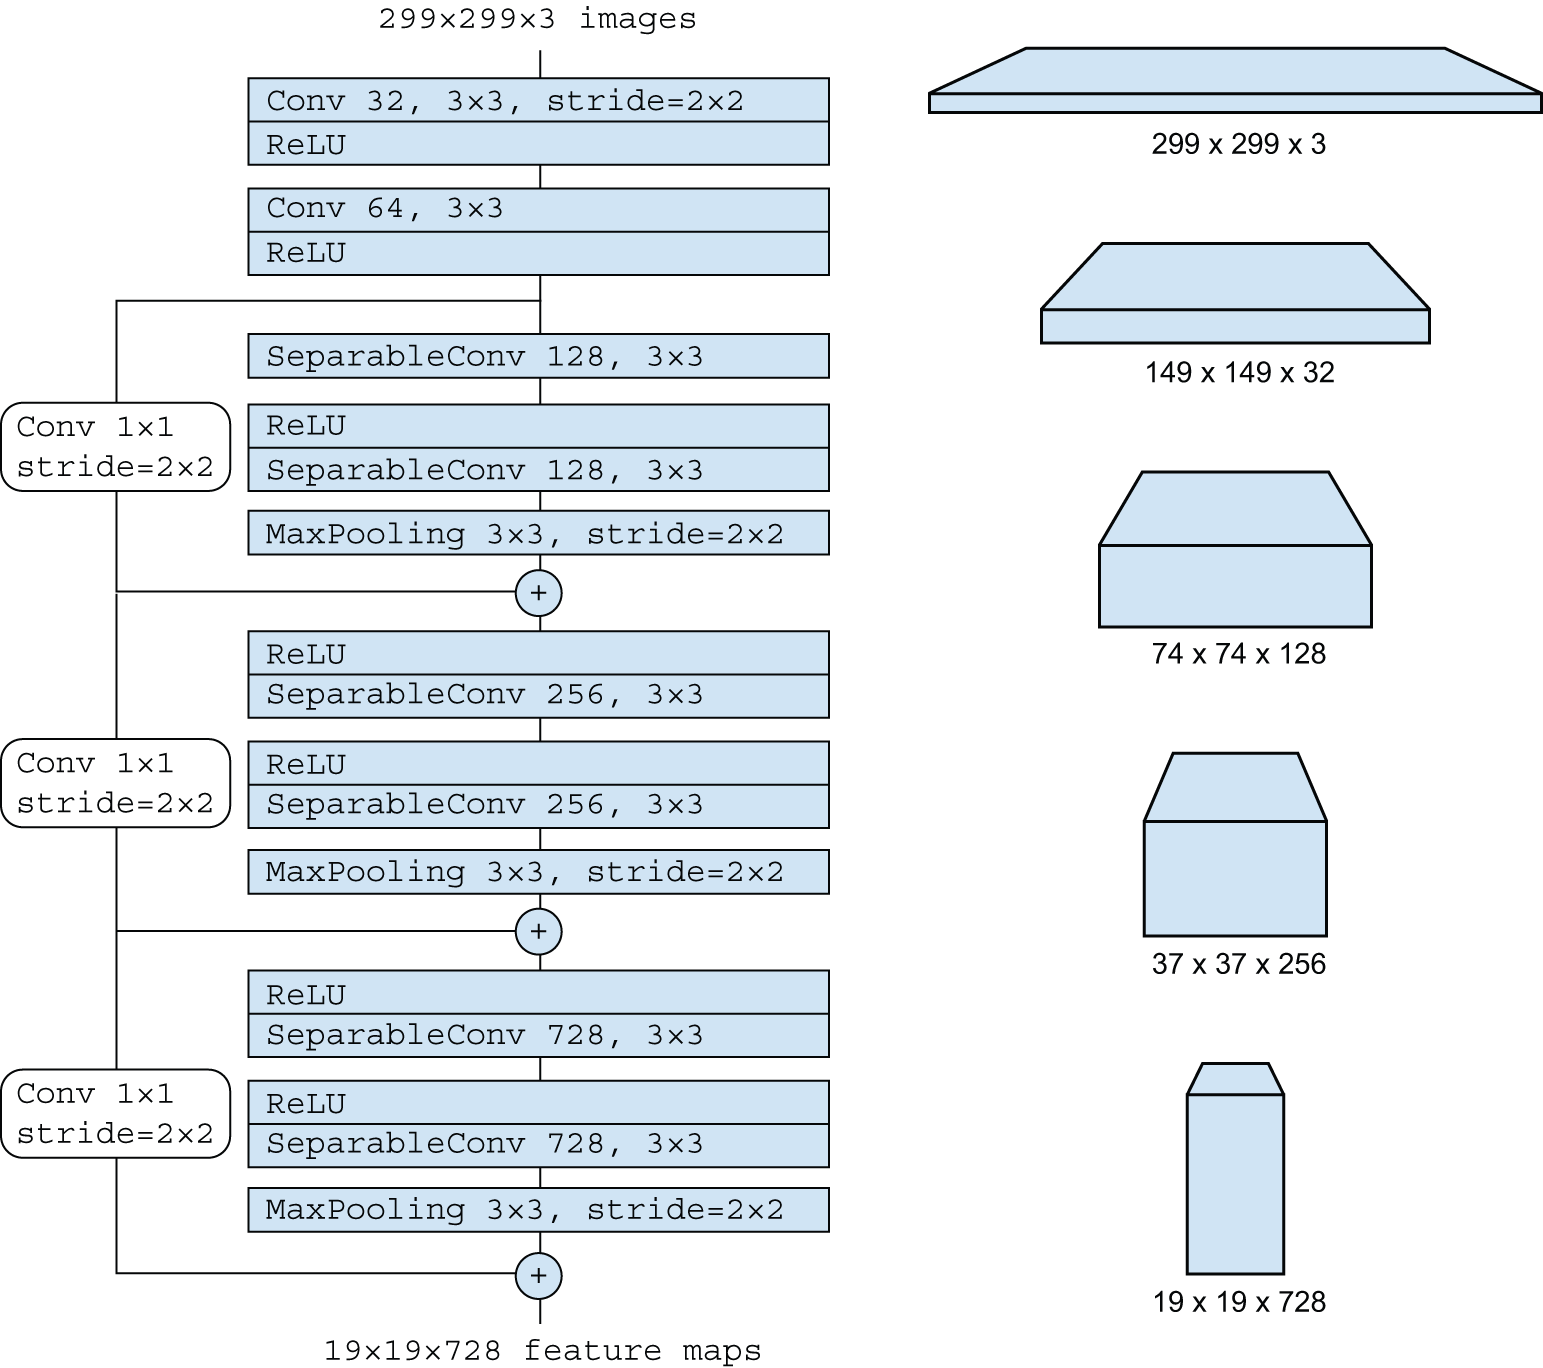
\includegraphics[width=\textwidth,height=0.7\textheight,keepaspectratio]{../../images/ch09/xception_entry_flow_pyramid.4701a5de.png}
            \caption{Sự phân cấp của Khối đầu vào Xception}
        \end{figure}
    \end{columns}
\end{frame}

\section{2. Kết nối Thặng dư (Residual Connections)}

\begin{frame}{Vấn đề: Suy biến Đạo hàm (Vanishing Gradient)}
    \begin{itemize}
        \item Mạng càng \textbf{Sâu (Deep)}, hệ thống phân cấp (Hierarchy) càng hiệu quả vì nó ép mô hình tạo ra các đặc trưng trừu tượng cao cấp (Abstraction).
        \item Trực giác mách bảo: Cứ xếp chồng thêm lớp, mô hình sẽ càng thông minh.
        \item Tuy nhiên, khi xếp chồng quá nhiều lớp (ví dụ: hàng trăm lớp Conv2D), mạng đột ngột \textbf{ngừng học}, Loss không suy giảm.
        \item Hiện tượng này không phải do Overfitting, mà do \textbf{Vanishing Gradient}.
    \end{itemize}
\end{frame}

\begin{frame}{Quy tắc Chuỗi (Chain Rule) và Trò chơi Truyền tin}
    \begin{itemize}
        \item Thuật toán Backpropagation truyền đạo hàm ngược từ hàm Loss về các tầng đầu thông qua \textbf{Quy tắc chuỗi (Chain Rule)}.
        \item Quá trình này giống như trò chơi \textit{Truyền tin tĩnh điện (Chinese Whispers/Telephone)}: Thông điệp qua từng người sẽ bị nhiễu dần.
        \item Phép nhân liên tiếp nhiều số nhỏ hơn 1 (qua các hàm \texttt{ReLU}, lớp Dropout) sẽ khiến đạo hàm giảm mạnh theo cấp số nhân về số 0.
        \item Các tầng đầu tiên không nhận được bất kỳ tín hiệu cập nhật nào, mô hình bị "tê liệt".
    \end{itemize}
\end{frame}

\begin{frame}{Giải pháp: Kết nối Thặng dư (Residual Connections)}
    \begin{columns}
        \column{0.5\textwidth}
        \begin{itemize}
            \item Phát minh của Kaiming He (2015) trong kiến trúc \textbf{ResNet} (Đạt giải Best Paper tại CVPR).
            \item Cung cấp một \textbf{đường tắt (Shortcut)} cho thông tin nhảy vọt qua khối tính toán (không bị biến đổi).
            \item Đầu vào được cộng trực tiếp vào đầu ra: $y = F(x) + x$.
            \item Đạo hàm chảy ngược xuyên qua các "đường cao tốc" này về đầu mạng một cách mượt mà.
        \end{itemize}
        
        \column{0.5\textwidth}
        \begin{figure}
            \centering
            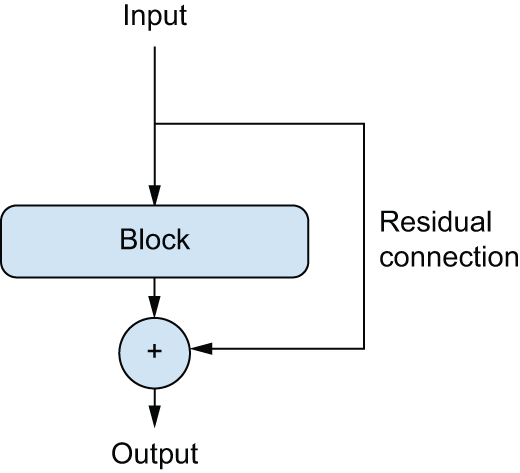
\includegraphics[width=\textwidth,height=0.7\textheight,keepaspectratio]{../../images/ch09/residual_connection.0524fdc4.png}
            \caption{Cơ chế hoạt động của Khối Residual}
        \end{figure}
    \end{columns}
\end{frame}

\begin{frame}[fragile]{Mã nguồn giả (Pseudocode) cho Residual}
Thay vì bắt khối (block) học ra một kết quả ánh xạ $F(x)$ hoàn toàn mới (rất khó), ta chỉ bắt nó học phần \textbf{thặng dư (Residual)} còn thiếu so với đầu vào. 

\begin{lstlisting}[language=Python]
# Some input tensor
x = ...
# Saves a reference to the original input. This is called the residual.
residual = x

# This computation block can potentially be destructive or noisy.
# It only needs to learn the "difference" (residual).
x = block(x)

# Adds the original input to the layer's output. The final output will
# thus always preserve full information about the original input.
x = add([x, residual])
\end{lstlisting}
\end{frame}

\begin{frame}[fragile]{Mã nguồn: Cân bằng số lượng Bộ lọc (Filters)}
Phép cộng \texttt{add([x, residual])} đòi hỏi 2 Tensor phải có cùng hình dáng (Shape). Khi Khối Convolution làm tăng số lượng Channels, ta phải dùng một lớp \texttt{Conv2D} $1 \times 1$ để chiếu (Project) đường dẫn thặng dư lên cùng số Channels.

\begin{lstlisting}[language=Python]
inputs = keras.Input(shape=(32, 32, 3))
x = layers.Conv2D(32, 3, activation="relu")(inputs)
residual = x

# Block increases output filters from 32 to 64
x = layers.Conv2D(64, 3, activation="relu", padding="same")(x)

# Project the residual using 1x1 Conv2D to match 64 filters
residual = layers.Conv2D(64, 1)(residual)

x = layers.add([x, residual])
\end{lstlisting}
\end{frame}

\begin{frame}[fragile]{Mã nguồn: Cân bằng Kích thước (MaxPooling)}
Tương tự, khi không gian bị thu nhỏ bởi \texttt{MaxPooling2D}, ta cũng phải thu nhỏ đường dẫn Residual bằng tham số \texttt{strides=2} để bảo đảm khớp kích thước khi cộng.

\begin{lstlisting}[language=Python]
inputs = keras.Input(shape=(32, 32, 3))
x = layers.Conv2D(32, 3, activation="relu")(inputs)
residual = x

# Block includes MaxPooling downsampling
x = layers.Conv2D(64, 3, activation="relu", padding="same")(x)
x = layers.MaxPooling2D(2, padding="same")(x)

# Project the residual and apply downsampling with strides=2
residual = layers.Conv2D(64, 1, strides=2)(residual)

x = layers.add([x, residual])
\end{lstlisting}
\end{frame}

\section{3. Batch Normalization (Chuẩn hóa Hàng loạt)}

\begin{frame}{Tại sao cần Chuẩn hóa Kích hoạt (Activation Normalization)?}
    \begin{itemize}
        \item Chuẩn hóa dữ liệu đầu vào (căn giữa Mean=0, tỷ lệ Variance=1) giúp mô hình dễ hội tụ. (Ví dụ: scale pixel từ 0-255 về 0-1).
        \item Nhưng khi dữ liệu đi sâu vào các lớp bên trong, sự phân bố liên tục bị biến đổi sau mỗi phép nhân ma trận.
        \item Các tầng phía sau liên tục phải thích nghi với dữ liệu đầu vào mới thay đổi liên tục. Sự bất ổn này gọi là \textbf{Internal Covariate Shift}.
        \item \textbf{Batch Normalization} (Ioffe \& Szegedy, 2015) giải quyết vấn đề bằng cách \textit{chuẩn hóa lại dữ liệu ngay trong lúc đang di chuyển} giữa các tầng.
    \end{itemize}
\end{frame}

\begin{frame}{Toán học của Batch Normalization}
    Lớp \texttt{BatchNormalization} chuẩn hóa từng lô (Batch) trong lúc Training:
    \begin{enumerate}
        \item Tính Kỳ vọng ($\mu$) của Batch: $\mu = \frac{1}{m} \sum_{i=1}^m x_i$
        \item Tính Phương sai ($\sigma^2$) của Batch: $\sigma^2 = \frac{1}{m} \sum_{i=1}^m (x_i - \mu)^2$
        \item Chuẩn hóa gốc: $\hat{x}_i = \frac{x_i - \mu}{\sqrt{\sigma^2 + \epsilon}}$
        \item \textbf{Dịch chuyển và Tỷ lệ (Scale \& Shift):} $y_i = \gamma \hat{x}_i + \beta$
    \end{enumerate}
    Trong đó, $\gamma$ và $\beta$ là 2 tham số \textbf{được học} qua Gradient Descent. Nó cho phép mô hình \textit{hủy bỏ} tác dụng của BN và khôi phục phân phối gốc nếu việc chuẩn hóa làm mất đi thông tin quý giá.
\end{frame}

\begin{frame}{Quá trình Suy luận (Inference Mode)}
    \begin{itemize}
        \item Khi Đưa vào sử dụng (Inference/Predict), ta thường dự đoán trên từng ảnh đơn lẻ (Batch Size = 1). Không thể tính $\mu$ và $\sigma^2$ của 1 ảnh được!
        \item Giải pháp: Trong suốt quá trình Training, lớp BN âm thầm cập nhật một \textbf{Trung bình động lũy thừa (Exponential Moving Average)} của các $\mu$ và $\sigma^2$ từ tất cả các batches.
        \item Khi Inference, nó dùng hằng số Moving Average này để chuẩn hóa thay vì tính toán lại.
        \item \textit{Lưu ý khi Transfer Learning:} Luôn đóng băng (Freeze) lớp BN bằng `trainable=False` để tránh làm hỏng Moving Average đã được học rất tốt từ ImageNet.
    \end{itemize}
\end{frame}

\begin{frame}[fragile]{Cách lập trình Batch Normalization chuẩn xác}
Vì BN tự động chuẩn hóa Mean về 0, tham số \texttt{bias} của tầng Convolution trước đó trở nên vô dụng (bị hấp thụ bởi $\beta$). Ta nên tắt nó bằng \texttt{use\_bias=False} để tiết kiệm RAM.

\textbf{Cách KHÔNG NÊN dùng (Activation bị đặt sai chỗ):}
\begin{lstlisting}[language=Python]
x = layers.Conv2D(32, 3, activation="relu")(x)
x = layers.BatchNormalization()(x)
\end{lstlisting}

\textbf{Cách SỬ DỤNG CHUẨN (BN phải đứng TRƯỚC Hàm kích hoạt):}
\begin{lstlisting}[language=Python]
# Note the lack of bias and activation here
x = layers.Conv2D(32, 3, use_bias=False)(x)
x = layers.BatchNormalization()(x)
# We place the activation AFTER the BatchNormalization layer
x = layers.Activation("relu")(x)
\end{lstlisting}
\end{frame}

\section{4. Tích chập Tách rời (Separable Convolution)}

\begin{frame}{Giới hạn của Tích chập Truyền thống (Conv2D)}
    \begin{itemize}
        \item Lớp \texttt{Conv2D} thực hiện đồng thời 2 việc trong 1 bước tính toán duy nhất:
        \begin{enumerate}
            \item Học các mẫu Không gian 2D (Spatial Pattern - VD: đường viền).
            \item Tổ hợp thông tin chéo từ nhiều Kênh (Cross-channel Mixing - VD: Kết hợp kênh Đỏ và Xanh).
        \end{enumerate}
        \item Chi phí tính toán cực kỳ tốn kém, số tham số: $K^2 \times C_{in} \times C_{out}$.
        \item \textbf{Giả thuyết mới:} Đặc trưng Không gian và Đặc trưng Kênh có tính độc lập cao. Tại sao không tách chúng ra?
    \end{itemize}
\end{frame}

\begin{frame}{Tích chập Tách rời (Depthwise Separable Convolution)}
    \begin{columns}
        \column{0.5\textwidth}
        Tách phép tính thành 2 pha độc lập (\texttt{SeparableConv2D}):
        \begin{enumerate}
            \item \textbf{Depthwise Conv:} Quét không gian trên từng Kênh một cách độc lập (Không trộn lẫn).
            \item \textbf{Pointwise Conv ($1 \times 1$):} Nhào trộn thông tin giữa các Kênh tại từng điểm ảnh.
        \end{enumerate}
        Số lượng tham số giảm mạnh: $K^2 \times C_{in} + C_{in} \times C_{out}$.
        
        \column{0.5\textwidth}
        \begin{figure}
            \centering
            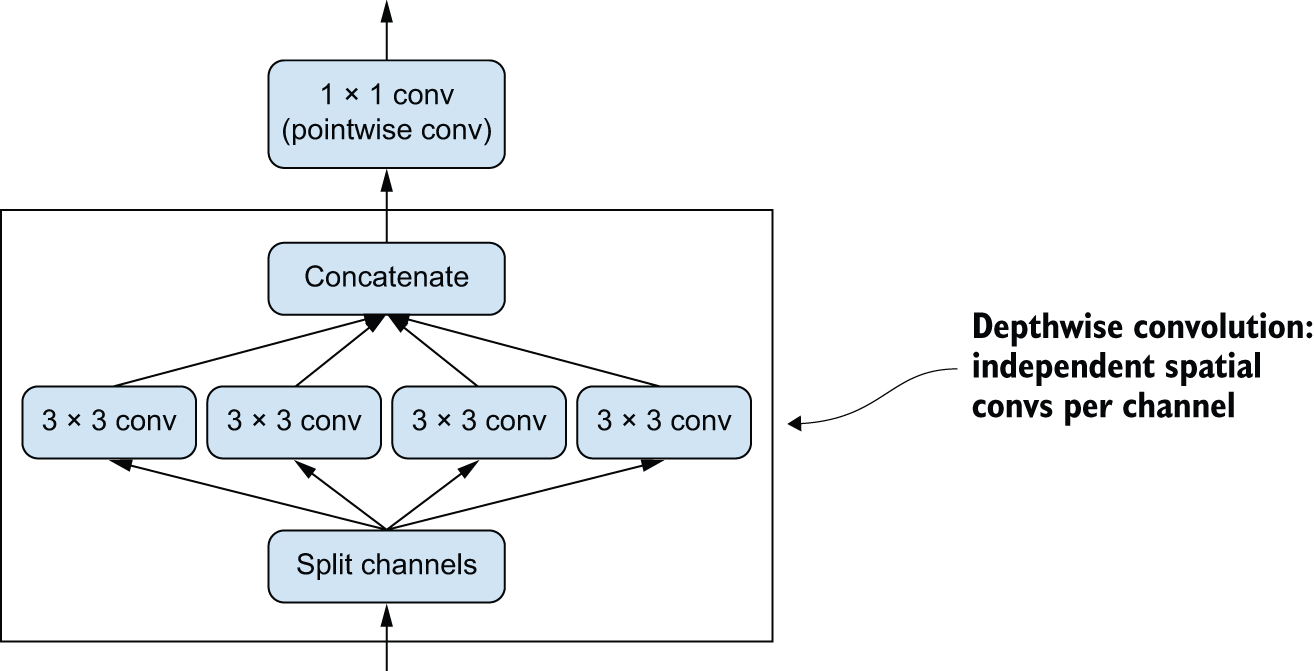
\includegraphics[width=\textwidth,height=0.7\textheight,keepaspectratio]{../../images/ch09/depthwise_separable_conv.5d1929bd.png}
            \caption{Tích chập Tách rời chiều sâu}
        \end{figure}
    \end{columns}
\end{frame}

\begin{frame}{Phân tích Toán học về Hiệu suất}
    \begin{itemize}
        \item Giả sử ta dùng Kernel $3 \times 3$, đầu vào có $64$ Channels, đầu ra có $64$ Channels.
        \item \textbf{Tích chập chuẩn (Conv2D):}
        \begin{itemize}
            \item Số tham số = $3^2 \times 64 \times 64 = 36,864$ tham số.
        \end{itemize}
        \item \textbf{Tích chập Tách rời (SeparableConv2D):}
        \begin{itemize}
            \item Số tham số = $(3^2 \times 64) + (64 \times 64) = 576 + 4,096 = 4,672$ tham số.
        \end{itemize}
        \item \textbf{Kết luận:} Tiết kiệm gần $90\%$ bộ nhớ và năng lực tính toán. Mô hình hội tụ nhanh hơn, chống Overfitting tốt hơn do ít tham số dư thừa.
    \end{itemize}
\end{frame}

\begin{frame}{Sự co-evolve (Tiến hóa đồng thời) của Phần cứng và Phần mềm}
    \begin{itemize}
        \item Dù tiết kiệm 90\% tham số, nhưng trên GPU thực tế, \texttt{SeparableConv2D} chỉ nhanh **tương đương** \texttt{Conv2D} thông thường. Tại sao?
        \item Bởi vì \textbf{NVIDIA cuDNN} đã tối ưu vi mô (micro-optimized) kernel \texttt{Conv2D} tiêu chuẩn bằng hợp ngữ (Assembly) qua hàng thập kỷ cho hàng Exaflops tính toán.
        \item Các thuật toán mới dù ưu việt về toán học nhưng không được phần cứng ưu tiên thiết kế $\rightarrow$ Sẽ chạy rất chậm.
        \item Đây là rào cản khổng lồ (Sự tiến hóa đồng thời của Hardware - Software - Algorithm) ngăn chặn các đột phá AI đi chệch khỏi lối mòn của Backpropagation.
    \end{itemize}
\end{frame}

\section{5. Thực hành: Xây dựng Mini-Xception}

\begin{frame}[fragile]{Lắp ráp mô hình Mini-Xception (Phần 1)}
Chương trình sau ứng dụng cả 3 bảo bối: \textbf{SeparableConv}, \textbf{BatchNormalization}, và \textbf{Residual Connections}.

\begin{lstlisting}[language=Python]
inputs = keras.Input(shape=(180, 180, 3))
x = layers.Rescaling(1.0 / 255)(inputs)

# First layer must be regular Conv2D because RGB channels 
# are highly correlated in natural images. Separable assumption fails here!
x = layers.Conv2D(filters=32, kernel_size=5, use_bias=False)(x)

for size in [32, 64, 128, 256, 512]:
    residual = x

    x = layers.BatchNormalization()(x)
    x = layers.Activation("relu")(x)
    x = layers.SeparableConv2D(size, 3, padding="same", use_bias=False)(x)
\end{lstlisting}
\end{frame}

\begin{frame}[fragile]{Lắp ráp mô hình Mini-Xception (Phần 2)}
Kết thúc vòng lặp, ta gắn khối Classifier (Toàn cục). Kích thước mạng cực nhẹ, chỉ tốn $721,857$ tham số so với 1.5 triệu tham số của CNN cũ!

\begin{lstlisting}[language=Python]
    x = layers.BatchNormalization()(x)
    x = layers.Activation("relu")(x)
    x = layers.SeparableConv2D(size, 3, padding="same", use_bias=False)(x)
    x = layers.MaxPooling2D(3, strides=2, padding="same")(x)

    # Project residual block
    residual = layers.Conv2D(size, 1, strides=2, padding="same", use_bias=False)(residual)
    x = layers.add([x, residual])

x = layers.GlobalAveragePooling2D()(x)
x = layers.Dropout(0.5)(x)
outputs = layers.Dense(1, activation="sigmoid")(x)
model = keras.Model(inputs=inputs, outputs=outputs)
\end{lstlisting}
\end{frame}

\begin{frame}{Đánh giá Độ chính xác (Accuracy)}
    \begin{columns}
        \column{0.5\textwidth}
        \begin{itemize}
            \item Nhờ cấu trúc siêu ưu việt, mô hình tự thiết kế của chúng ta đạt \textbf{Accuracy lên đến 90.8\%} trên tập Chó/Mèo.
            \item Mô hình Basic CNN ở Chương 8 (Không dùng Transfer Learning) chỉ đạt được mốc 83.9\%.
            \item Thiết kế kiến trúc chuẩn mực (Architecture Best Practices) mang lại \textbf{Bước nhảy vọt} về hiệu năng!
        \end{itemize}
        
        \column{0.5\textwidth}
        \begin{figure}
            \centering
            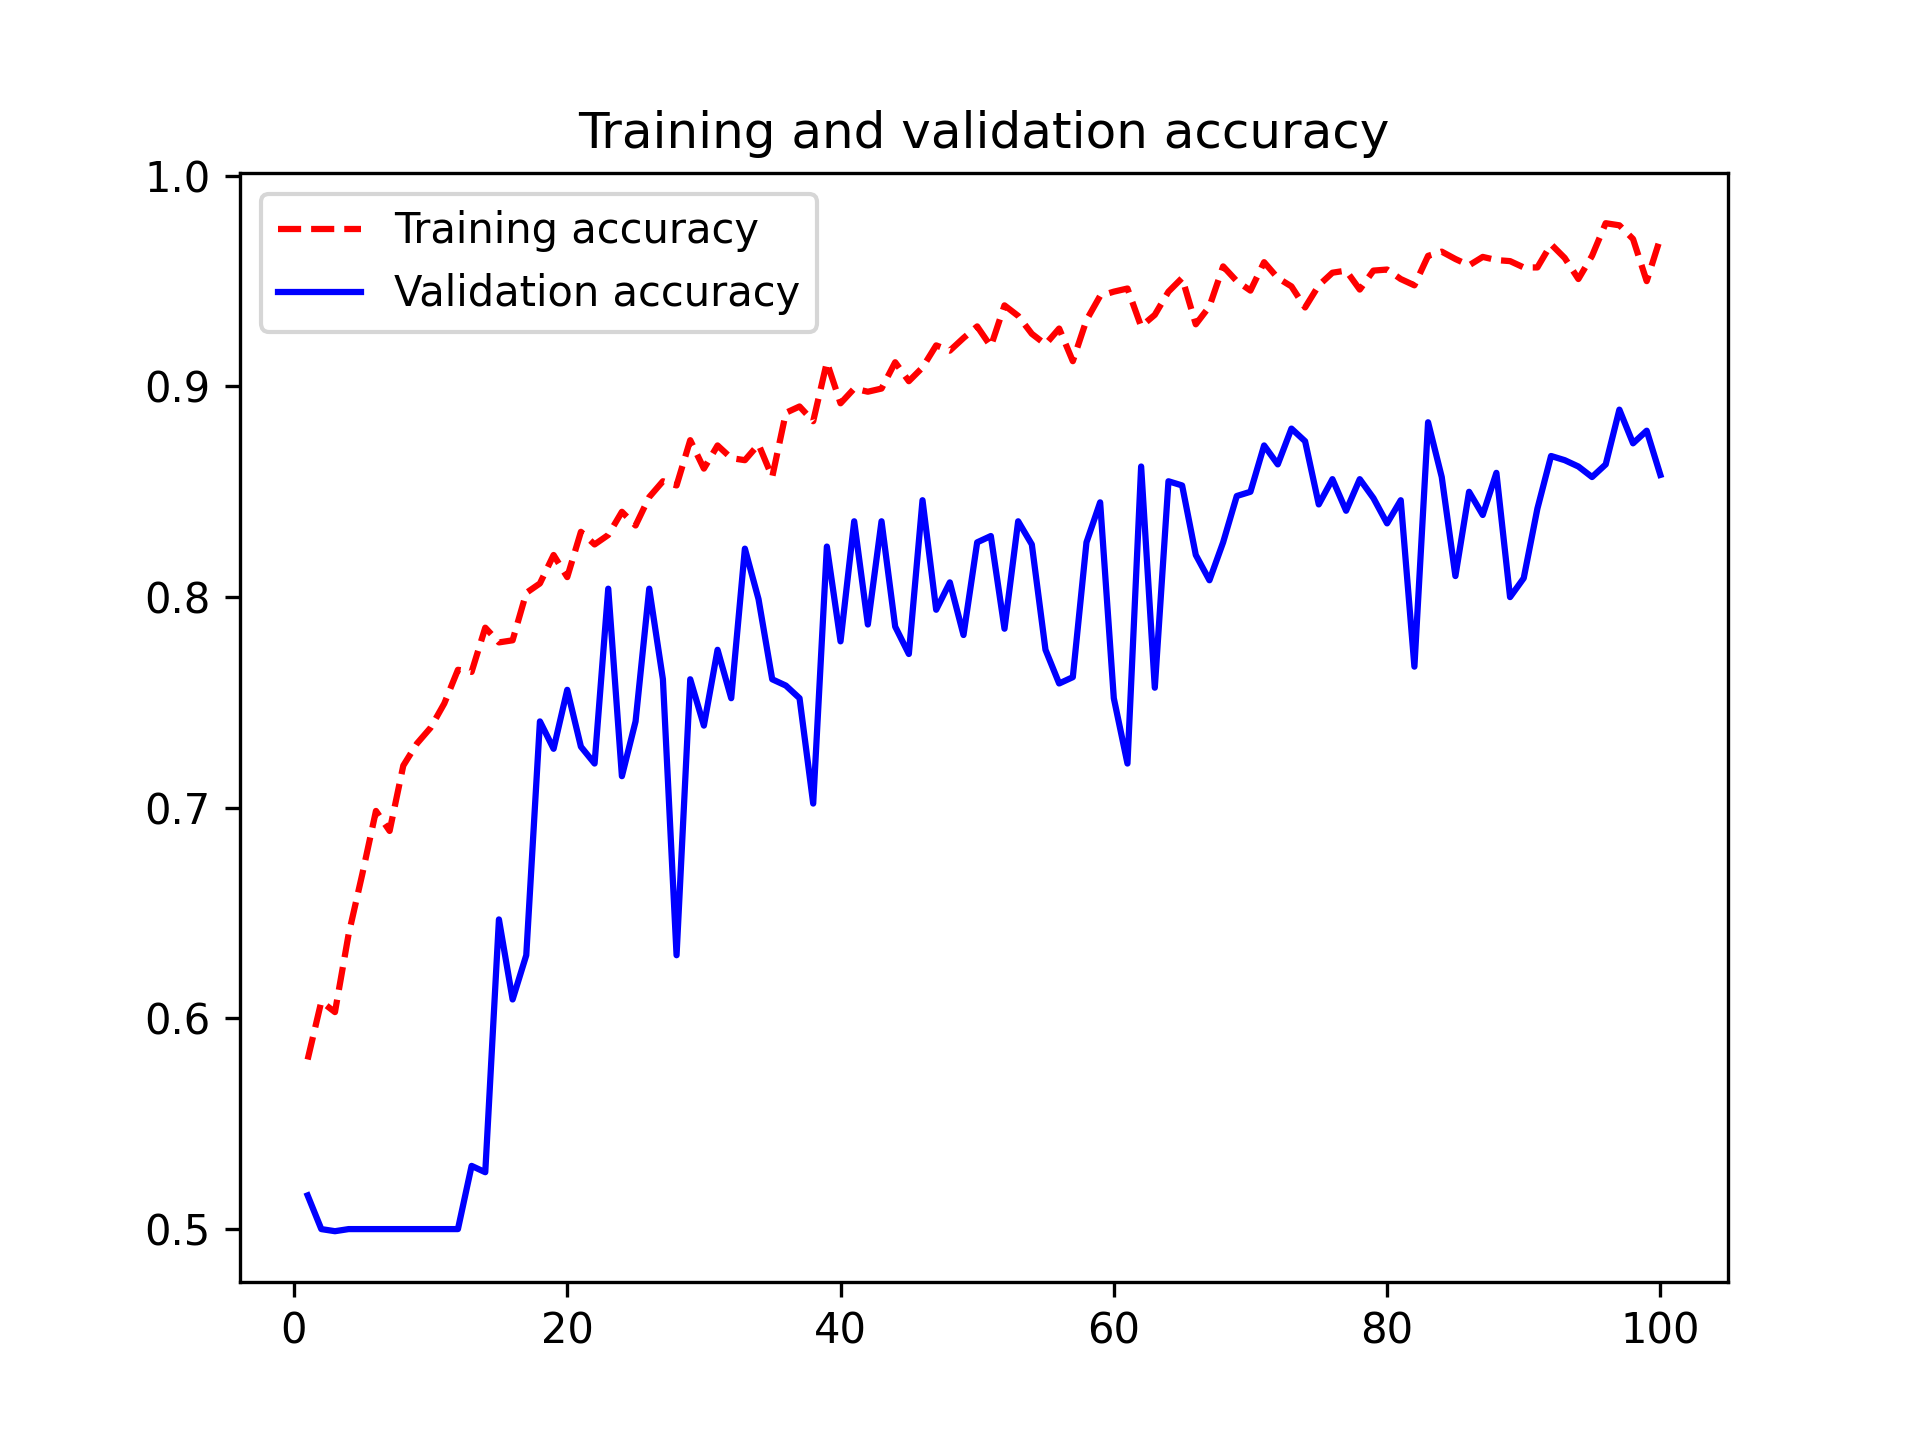
\includegraphics[width=\textwidth,height=0.5\textheight,keepaspectratio]{../../images/ch09/training-and-validation-xception-acc.967bf65c.png}
            \caption{Accuracy của Mini-Xception}
        \end{figure}
    \end{columns}
\end{frame}

\begin{frame}{Đánh giá Mất mát (Loss)}
    \begin{columns}
        \column{0.5\textwidth}
        \begin{itemize}
            \item Đường Validation Loss đi xuống ổn định và mượt mà hơn.
            \item Sự hiện diện của \texttt{BatchNormalization} ở mọi ngõ ngách giúp thuật toán hội tụ cực nhanh.
            \item Dạng kiến trúc lặp (Xception) hiện là tiêu chuẩn công nghiệp (Industry Standard) trên Keras.
        \end{itemize}
        
        \column{0.5\textwidth}
        \begin{figure}
            \centering
            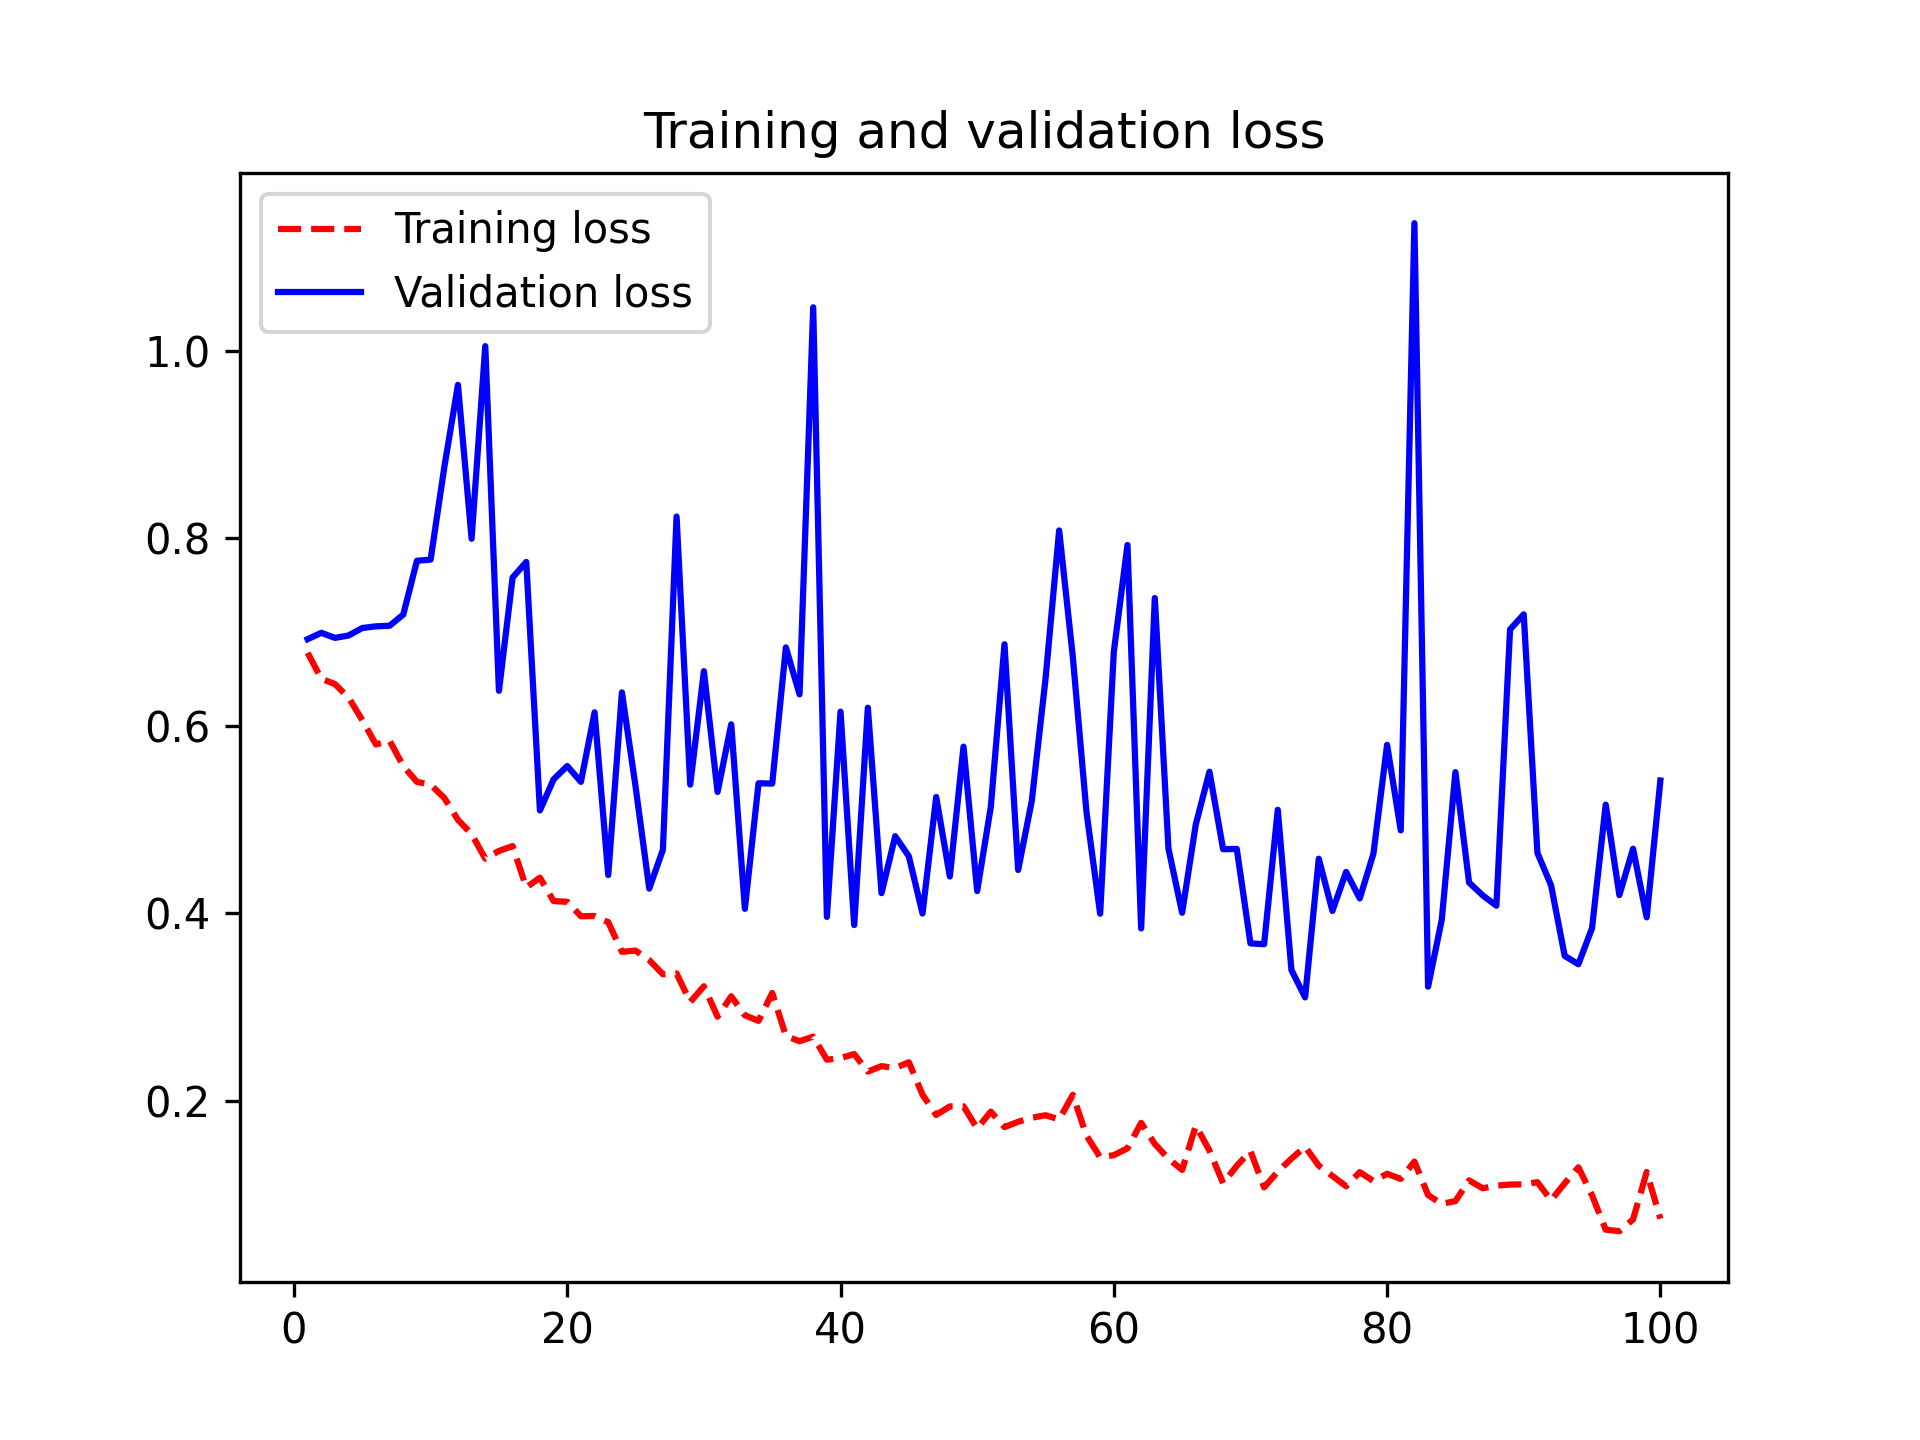
\includegraphics[width=\textwidth,height=0.5\textheight,keepaspectratio]{../../images/ch09/training-and-validation-xception-loss.bc0f5982.png}
            \caption{Loss của Mini-Xception}
        \end{figure}
    \end{columns}
\end{frame}

\section{6. Kỷ nguyên mới: Vision Transformers (ViTs)}

\begin{frame}{Giao thời của Công nghệ (Beyond Convolution)}
    \begin{itemize}
        \item Mạng Tích chập (ConvNets) đã độc tôn thống trị lĩnh vực Thị giác Máy tính suốt từ thập niên 2010.
        \item Gần đây, một Kiến trúc hoàn toàn mới đang đe dọa thay thế ngôi vương này: \textbf{Vision Transformers (ViTs)}.
        \item Transformers vốn dĩ được sinh ra vào năm 2017 dành riêng cho Xử lý Ngôn ngữ Tự nhiên (NLP - để dịch thuật văn bản).
        \item Ý tưởng táo bạo: Chuyện gì sẽ xảy ra nếu ta coi một bức ảnh giống như là "Một câu văn", và các bộ phận của ảnh là "Các từ vựng"?
    \end{itemize}
\end{frame}

\begin{frame}{Nguyên lý Hoạt động của ViTs}
    \begin{itemize}
        \item Mạng ViT hoàn toàn \textbf{bác bỏ} toán tử \texttt{Conv2D} để quét ảnh.
        \item Nó chặt bức ảnh gốc thành một lưới các mảnh ghép (Patches) có kích thước cố định, ví dụ $16 \times 16$ pixel.
        \item Trải phẳng mỗi mảnh ghép thành một Vector 1 chiều (Biến nó thành một "Từ vựng" - Token).
        \item Bơm toàn bộ chuỗi Vector vào kiến trúc Transformer để dùng cơ chế \textbf{Self-Attention} tìm kiếm mối tương quan.
    \end{itemize}
\end{frame}

\begin{frame}{Sức mạnh của Self-Attention}
    \begin{itemize}
        \item Mạng ConvNet gặp khó khăn trong việc kết nối các chi tiết ở xa nhau trên ảnh do kích thước Kernel ($3 \times 3$) quá nhỏ bé. Phải xếp lớp rất sâu mới nhìn được toàn cảnh.
        \item Mạng ViT với cơ chế Self-Attention có khả năng so sánh \textbf{mọi Patch với mọi Patch khác} cùng một lúc.
        \item Điều này tạo ra khả năng liên kết cự ly xa (Long-range relationships) tuyệt vời. Nó hiểu ngay lập tức quả bóng ở góc trái có liên quan mật thiết đến con chó đang chạy ở góc phải bức ảnh.
    \end{itemize}
\end{frame}

\begin{frame}{Hạn chế của ViTs so với ConvNets}
    Tuy rất mạnh, ViTs có những điểm yếu chí mạng đối với các dự án thực tế:
    \begin{itemize}
        \item \textbf{Cần dữ liệu khổng lồ:} ConvNets có lợi thế "Kiến thức ưu tiên 2D" (Biết rõ các pixel cạnh nhau thì liên quan đến nhau). ViTs là một tờ giấy trắng, nó phải tự học lại định luật vật lý về không gian $\rightarrow$ Phải đào tạo trên lượng dữ liệu khổng lồ (Lớn hơn cả ImageNet).
        \item \textbf{Mô hình quá đồ sộ:} Mạng ViT cực nặng, đòi hỏi hạ tầng Siêu máy tính (Clusters of TPUs/GPUs) khổng lồ để huấn luyện.
        \item Do đó, với các bài toán doanh nghiệp thông thường và dữ liệu có giới hạn, \textbf{ConvNets vẫn là sự lựa chọn hoàn hảo nhất.}
    \end{itemize}
\end{frame}

\section{Tổng kết}

\begin{frame}{Tổng kết Chương 9}
    Để xây dựng một mô hình CNN xuất sắc từ con số 0, hãy tuân theo các nguyên tắc sau:
    \begin{itemize}
        \item Tổ chức Mô hình theo dạng Tháp Đặc trưng (Feature Pyramid). Lặp lại Khối (Blocks) thay vì tự nối từng Layer ngẫu nhiên (Quy tắc MHR).
        \item Sử dụng \textbf{Separable Convolution} thay cho Convolution tiêu chuẩn (Tiết kiệm 90\% năng lực tính toán).
        \item Kết hợp \textbf{Batch Normalization} ngay trước Hàm Kích hoạt để hệ thống hội tụ mượt mà, triệt tiêu Covariate Shift.
        \item Tạo các \textbf{Kết nối Thặng dư (Residual Connections)} để dòng chảy Gradient truyền xa xuyên suốt mạng sâu hàng trăm tầng mà không bị suy biến.
    \end{itemize}
\end{frame}

\end{document}
